% Chapter Template

\chapter{Ensayos y resultados} % Main chapter title

\label{Chapter4} % Change X to a consecutive number; for referencing this chapter elsewhere, use \ref{ChapterX}

%----------------------------------------------------------------------------------------
%	SECTION 1
%----------------------------------------------------------------------------------------
En este capítulo se explica la metodología de pruebas aplicada tanto a los componentes individuales como al sistema implementado para finalizar con una comparación con el estado del arte.


\section{Banco de pruebas}
\label{sec:Banco de pruebas}
%
La verificación del correcto funcionamiento de los módulos que componen el sistema se realizó mediante una maqueta que se muestra en la figura \ref{fig:maqueta} y representa en escala reducida al invernadero del cliente.

El modelo cuenta con una bomba de agua conectada a tres válvulas para alimentar a los circuitos de riego. 
Se utilizaron mangueras y conexiones neumáticas de aluminio de acople rápido y el conjunto armado puede verse en la figura \ref{fig:pump}. 
  
El ensamblado se muestra en las figuras \ref{fig:gh1}, \ref{fig:gh2} y \ref{fig:gh3} donde se observa la implementación de dos circuitos de riego independientes. También se configuró un tercer circuito cerrado para pruebas de accionamiento de bomba y válvula a fin de evitar desperdicios durante las fases de calibración.


\begin{figure}[h]
	\centering
	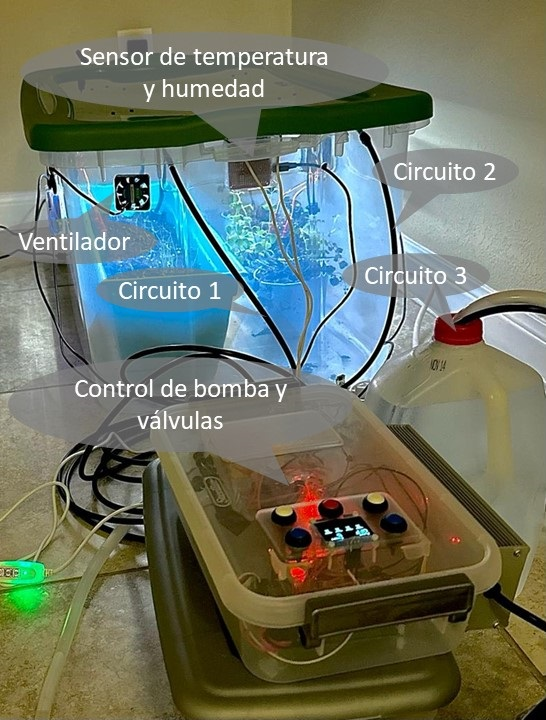
\includegraphics[width=0.50\textwidth]{./Figures/chapter4/maqueta.jpg}
	\caption[Modelo completo del invernadero]{Modelo completo del invernadero.}
	\label{fig:maqueta}
\end{figure}

Además se incorporaron a la maqueta dos módulos sensores de humedad del suelo, uno de temperatura y humedad y un actuador para el encendido de los ventiladores.

Para las pruebas manuales de accionamiento de los diferentes sistemas se empleó una computadora portátil y un celular para las pruebas de acceso concurrente a la aplicación central.

\begin{figure}[htpb]
     \centering
       \begin{subfigure}[b]{0.45\textwidth}
	    \centering
		 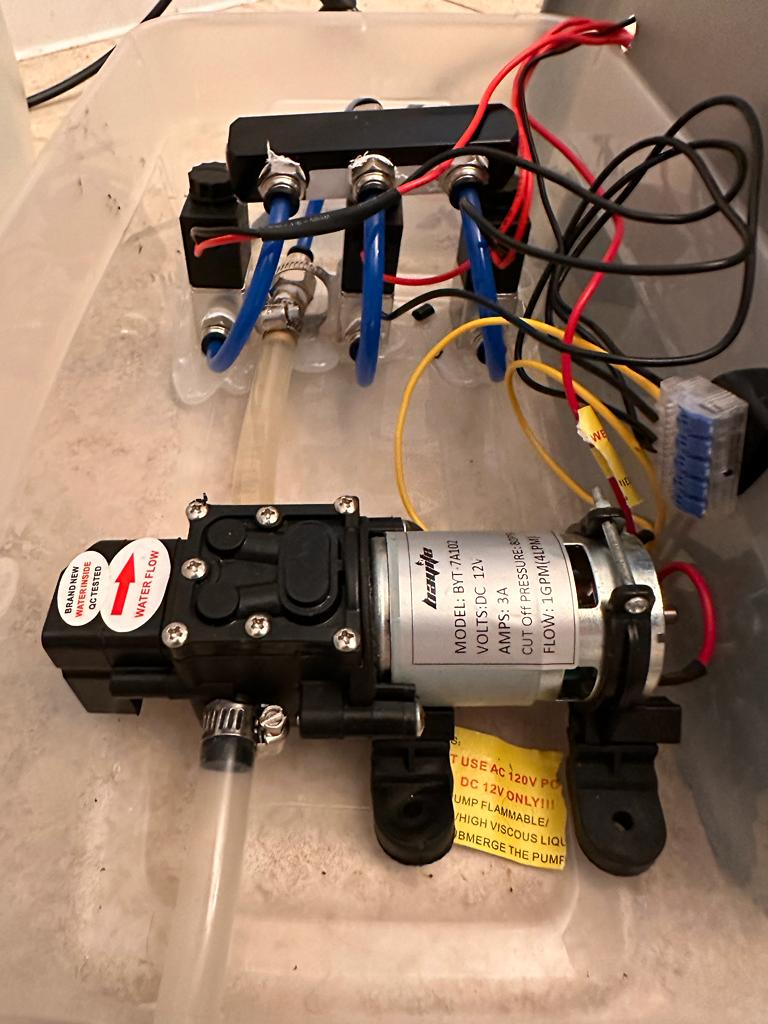
\includegraphics[width=0.75\textwidth]{./Figures/chapter4/pump_2.jpg}
		\caption{Conjunto bomba y válvulas.}
		\label{fig:pump}
     \end{subfigure}
          \hfill
     \begin{subfigure}[b]{0.45\textwidth}
		\centering
		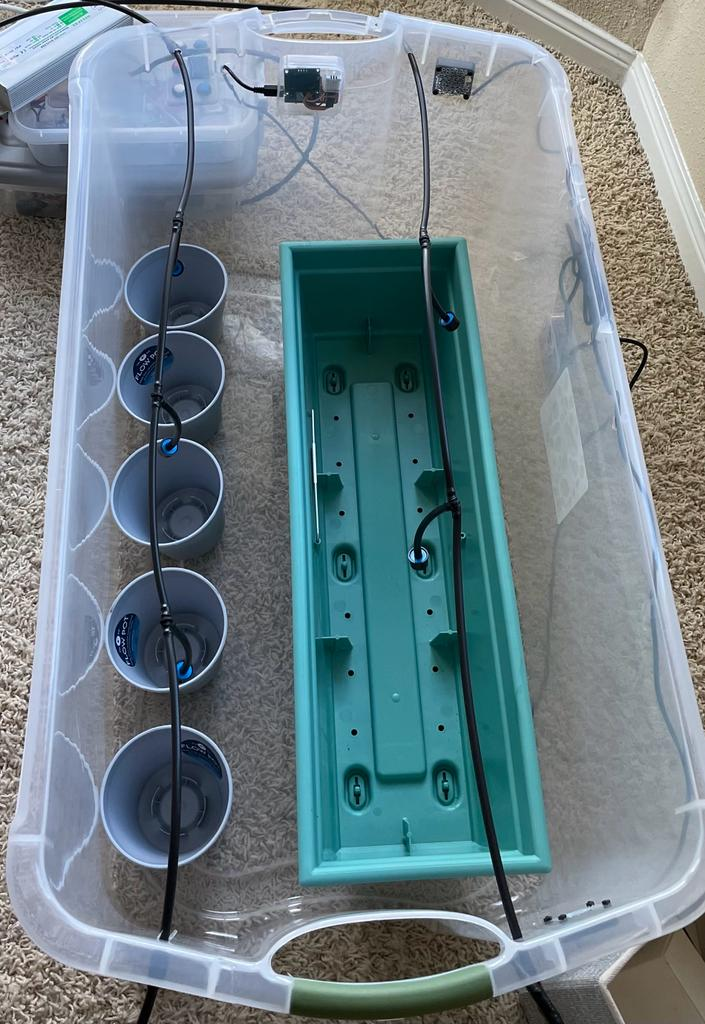
\includegraphics[width=0.70\textwidth]{./Figures/chapter4/Invernadero1.jpg}
		\caption{Armado de mangueras de riego.}
		\label{fig:gh1}
     \end{subfigure}
     \hfill
     \begin{subfigure}[b]{0.45\textwidth}
	    \centering
		 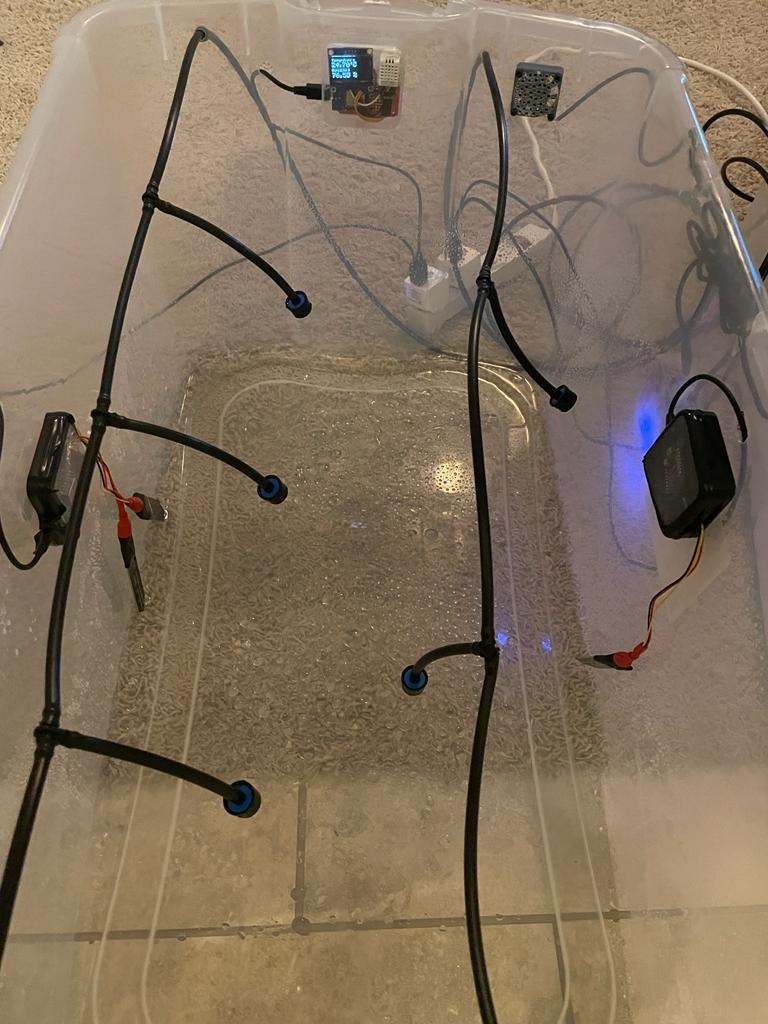
\includegraphics[width=0.75\textwidth]{./Figures/chapter4/Invernadero2.jpg}
		\caption{Pruebas de riego.}
		\label{fig:gh2}
     \end{subfigure}
     \hfill	
	 \begin{subfigure}[b]{0.45\textwidth}
		\centering
		\includegraphics[width=0.65\textwidth]{./Figures/chapter4/Invernadero3.jpg}
		\caption{Ensamble general.}
		\label{fig:gh3}
     \end{subfigure}
     \hfill

        \caption[Modelo de pruebas del invernadero]{Modelo de pruebas del invernadero.}
        \label{fig:invernadero}
\end{figure}



\pagebreak
\section{Pruebas unitarias}
\label{sec:Pruebas unitarias}

A continuación se detallan las principales pruebas realizadas a los módulos durante la fase de construcción del prototipo a fin de garantizar su correcto funcionamiento o el cumplimiento de requerimientos no funcionales.


\subsection{Pruebas a módulos sensores}
\label{sec:Pruebas a módulos sensores}

\begin{itemize}
\item Conexión a sensores y de su correcta lectura: Con el módulo conectado a la computadora principal se procedió a reportar por la consola serial los diferentes valores leídos. Se expuso a los sensores a diferentes condiciones, como por ejemplo mayor temperatura para el sensor de clima, o sumergirlo en agua al de humedad de suelo, y se corrobora que las mediciones reflejan los cambios realizados.
\item Resistencia al agua y a salpicaduras: Requerimiento no funcional explícito en el proyecto para los sensores de humedad del suelo, se procedió a realizar una medición continua de los mismos, al tiempo que se sumergieron los sensores en un recipiente con agua, luego se procedió a realizar aspersiones continuas por alrededor de 30 segundos con  atomizadores en diferentes ángulos. 
\end{itemize}
En la figura \ref{fig:soil_test} se observan los distintos elementos que conformaron las pruebas para los sensores de humedad del suelo.

\begin{figure}[h]
	\centering
	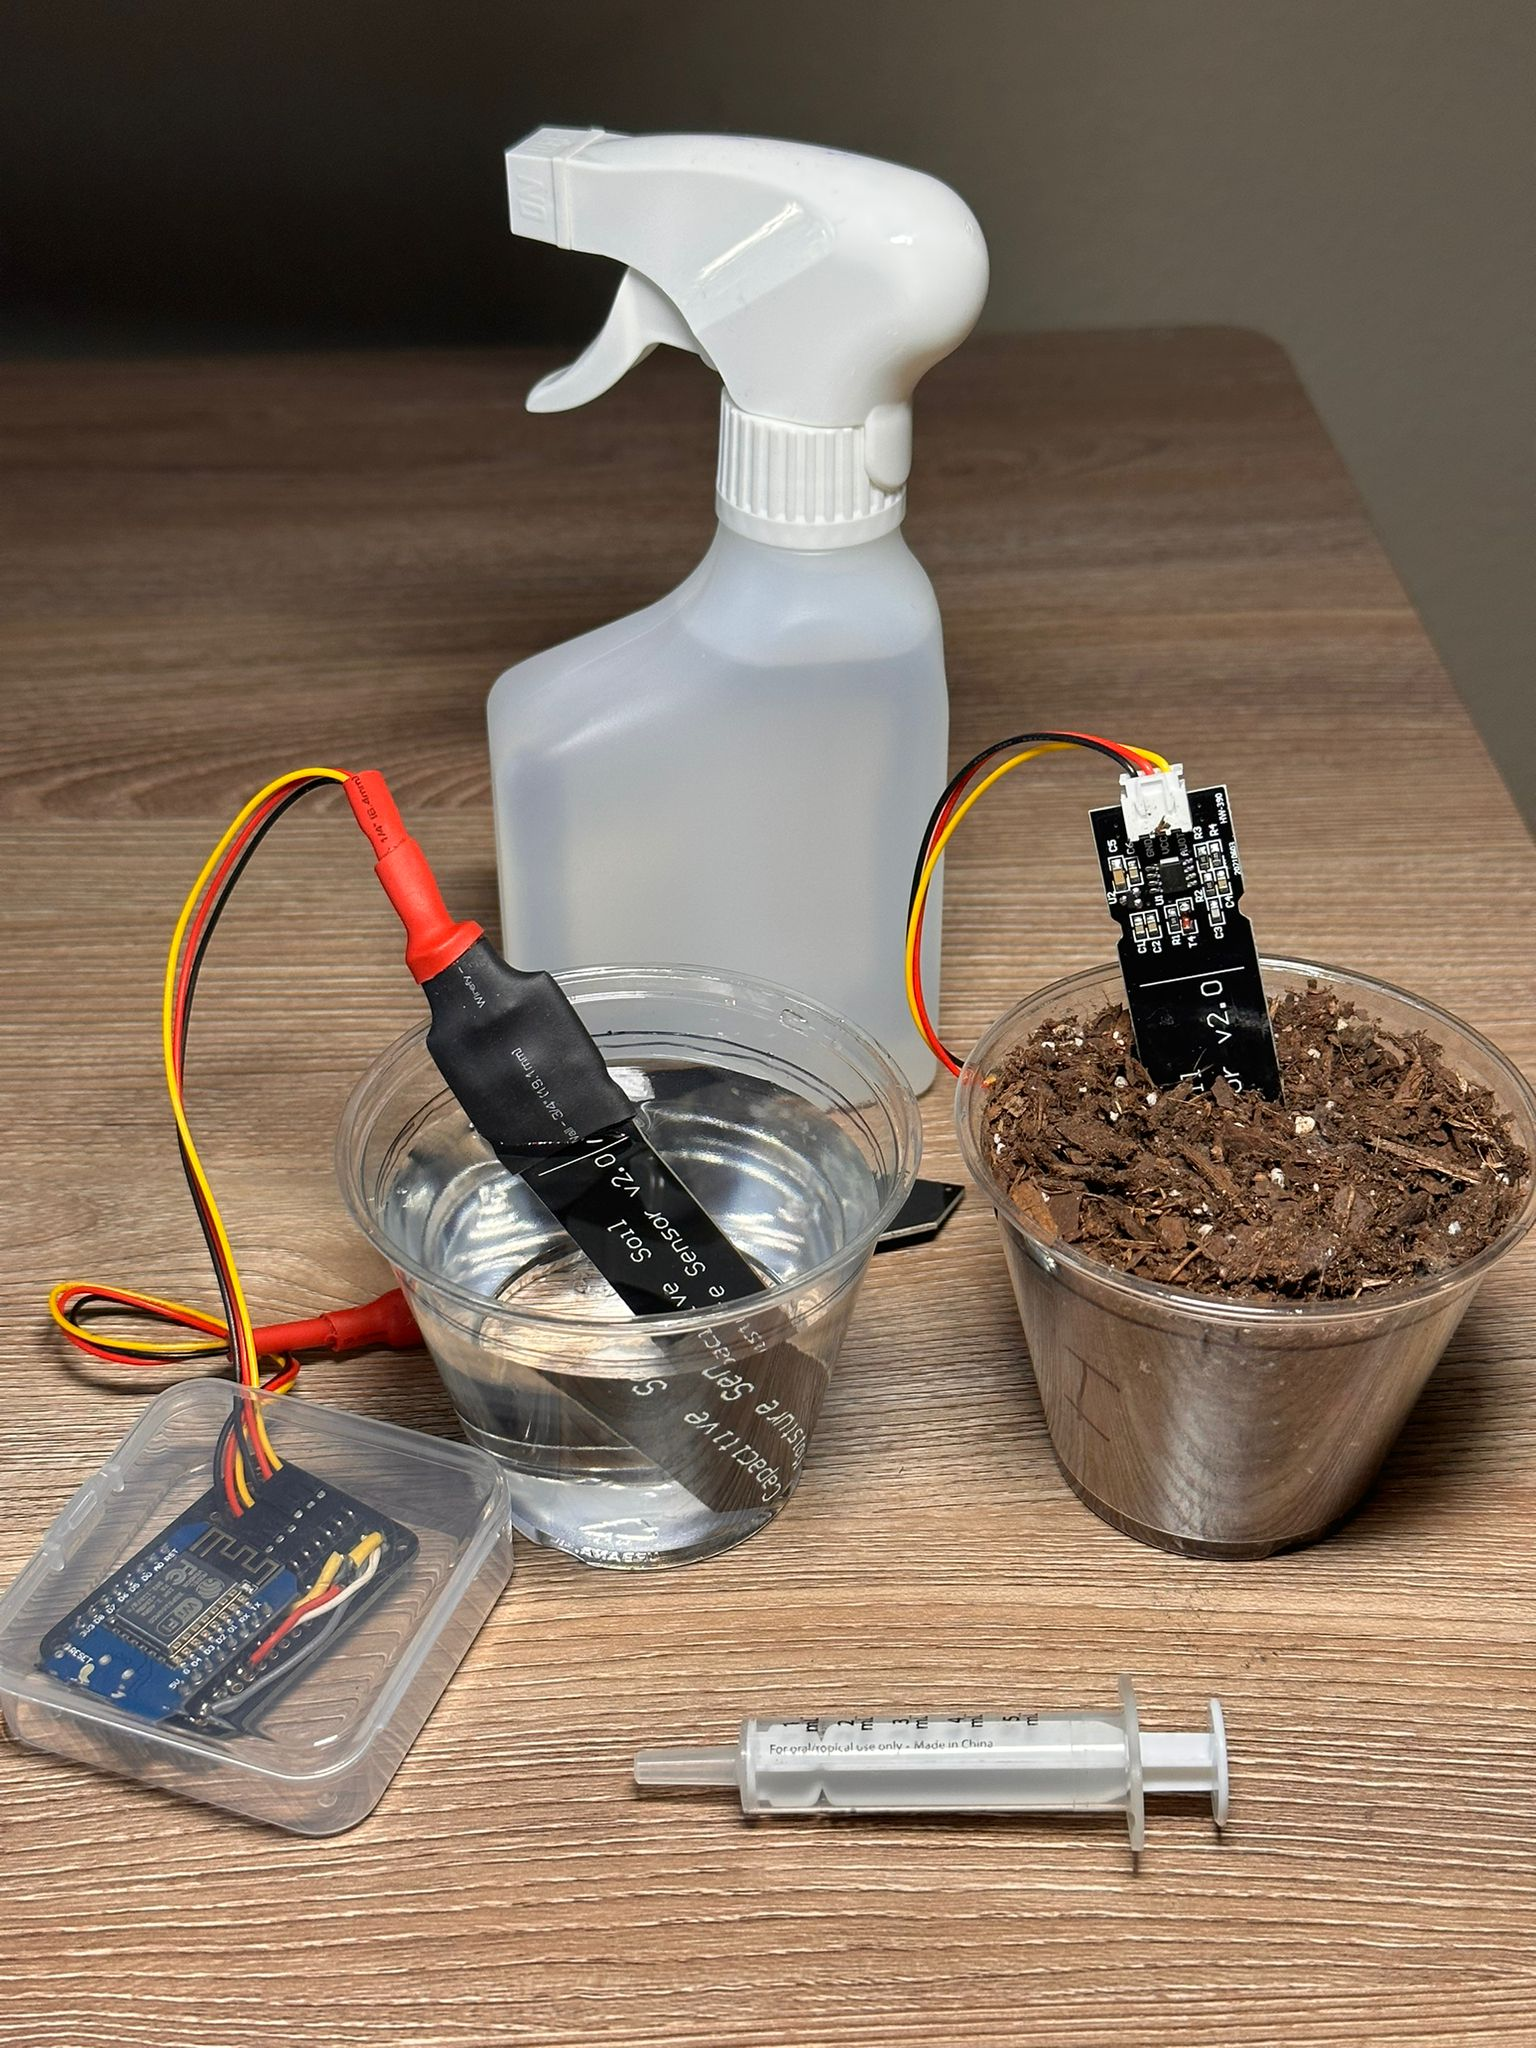
\includegraphics[width=0.50\textwidth]{./Figures/chapter4/soil_testing.jpg}
	\caption[Elementos para las pruebas de sensores de humedad del suelo]{Elementos para las pruebas de sensores de humedad del suelo.}
	\label{fig:soil_test}
\end{figure}

\subsection{Pruebas a módulos actuadores}
\label{sec:Pruebas a módulos actuadores}


\begin{itemize} 
\item Correcto accionamiento de sistemas: Se conectaron las salidas de los pines de GPIO mediante el uso de leds y resistencias para corroborar el correcto encendido o apagado de los mismos. Para la activación de estos, se desarrolló una interfaz simple en ThingsBoard que emita las señales de encendido y apagado por comandos RPC sobre MQTT. El microcontrolador, al subscribirse a los canales correspondientes recibe la señal y confirma la acción al prender or apagar los leds.
\end{itemize}


\begin{figure}[htpb]
     \centering
       \begin{subfigure}[b]{0.45\textwidth}
	    \centering
		 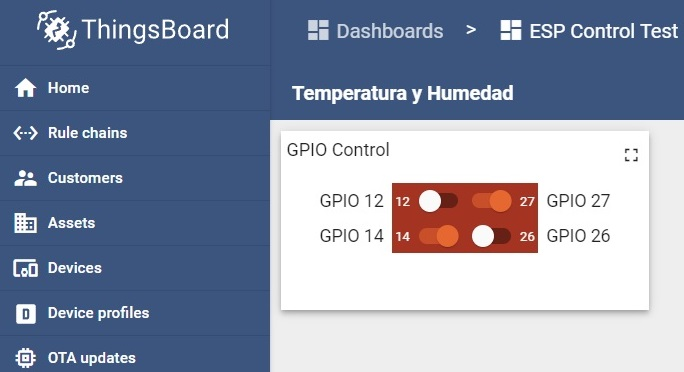
\includegraphics[width=0.9\textwidth]{./Figures/chapter4/control_unit_test_1.jpg}
		\caption{Ventana de control.}
		\label{fig:control_test1}
     \end{subfigure}
          \hfill
     \begin{subfigure}[b]{0.45\textwidth}
		\centering
		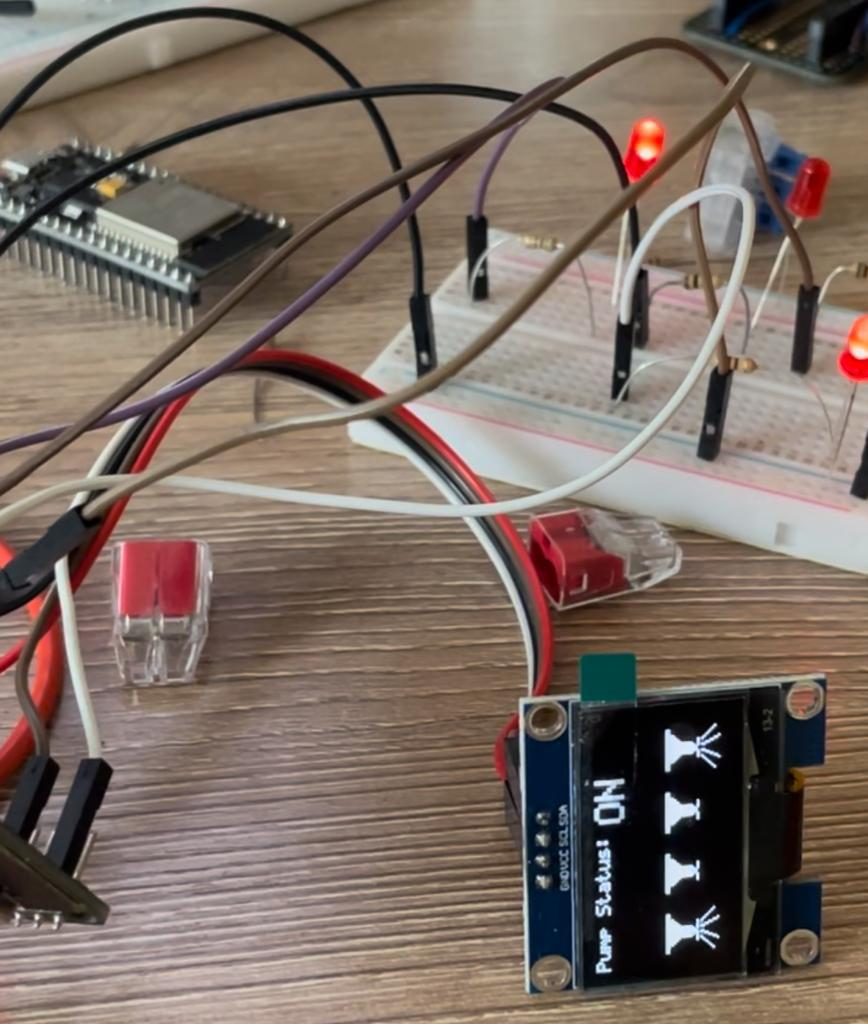
\includegraphics[width=0.70\textwidth]{./Figures/chapter4/control_test.jpg}
		\caption{Verificación de encendido de leds.}
		\label{fig:control_test1}
     \end{subfigure}
     \hfill
        \caption[Pruebas unitarias sobre controladores]{Pruebas unitarias sobre controladores.}
        \label{fig:control_test}
\end{figure}


\section{Pruebas de sistema}
\label{sec:Pruebas de sistema}

\textcolor{gray} {Aquí se describen las pruebas de sistema en donde interactúan dos o más componentes}


\section{Comparativa con el estado de arte}
\label{sec:Comparativa con el estado de arte}

\textcolor{gray} {Aquí se describe la comparación entre el modelo armado y lo informado en el capítulo 1}